\documentclass[10pt]{report}% ===> this file was generated automatically by noweave --- better not edit it
\usepackage{noweb}
\usepackage{graphicx}

\usepackage[table,dvipsnames]{xcolor}
\definecolor{apple_white}{rgb}{0.9,0.9,0.9}
\def \bk0 {\cellcolor{black}}
\def \bl0 {\cellcolor{Cerulean}}
\def \bw0 {\cellcolor{apple_white}}
\def \bo0 {\cellcolor{orange}}

\usepackage {booktabs}
\usepackage {tikz}
\usetikzlibrary {positioning, shapes.geometric, svg.path}

\noweboptions {smallcode,longchunks}

% Generate assembly file with:
% notangle -Rpreamble main.nw > main.asm
%
% Generate tex file with:
% noweave -delay -index main.nw > main.tex
% pdflatex main.tex (run twice for two passes)
% Indents in code only appears in the PDF output
% under TeX Live 2019.
%
% See also: https://www.cs.tufts.edu/~nr/noweb/johnson-lj.pdf

\begin{document}
\pagestyle{noweb}

\nwfilename{main.nw}\nwbegindocs{1}\chapter{Lode Runner}

\section{Introduction}
For dasm, we'll first specify that we're targeting the 6502 processor:

\nwenddocs{}\nwbegincode{2}\sublabel{NW1Xx3lK-1jwKhK-1}\nwmargintag{{\nwtagstyle{}\subpageref{NW1Xx3lK-1jwKhK-1}}}\moddef{preamble~{\nwtagstyle{}\subpageref{NW1Xx3lK-1jwKhK-1}}}\endmoddef\nwstartdeflinemarkup\nwusesondefline{\\{NW1Xx3lK-1p0Y9w-1}}\nwenddeflinemarkup
    PROCESSOR 6502
\nwused{\\{NW1Xx3lK-1p0Y9w-1}}\nwendcode{}\nwbegindocs{3}That is all!

\chapter{Apple II Graphics}
Hi-res graphics on the Apple II is odd. Graphics are memory-mapped, not exactly
consecutively, and bits don't always correspond to pixels. Color especially is
odd, compared to today's luxurious 32-bit per pixel RGBA.

\section{Pixels and their color}
First we'll talk about pixels. Nominally, the resolution of the hi-res graphics screen
is 280 pixels wide by 192 pixels tall. In the memory map, each row is represented
by 40 bytes. The high bit of each byte is not used for pixel data, but is used to
control color.

Here are some rules for how these bytes are turned into pixels:
\begin{itemize}
  \item Pixels are drawn to the screen from byte data least significant bit first.
        This means that for the first byte bit 0 is column 0, bit 1 is column 1,
        and so on.
  \item A pattern of {\Tt{}11\nwendquote} results in two white pixels at the {\Tt{}1\nwendquote} positions.
  \item A pattern of {\Tt{}010\nwendquote} results at least in a colored pixel at the {\Tt{}1\nwendquote} position.
  \item A pattern of {\Tt{}101\nwendquote} results at least in a colored pixel at the {\Tt{}0\nwendquote} position.
  \item So, a pattern of {\Tt{}01010\nwendquote} results in at least three consecutive colored
        pixels starting from the first {\Tt{}1\nwendquote} to the last {\Tt{}1\nwendquote}. The last {\Tt{}0\nwendquote} bit
        would also be colored if followed by a {\Tt{}1\nwendquote}.
  \item Likewise, a pattern of {\Tt{}11011\nwendquote} results in two white pixels, a colored pixel,
        and then two more white pixels.
  \item The color of a {\Tt{}010\nwendquote} pixel depends on the column that the {\Tt{}1\nwendquote} falls on, and
        also whether the high bit of its byte was set or not. 
  \item The color of a {\Tt{}11011\nwendquote} pixel depends on the column that the {\Tt{}0\nwendquote} falls on, and
        also whether the high bit of its byte was set or not.

        \begin{center}
        \begin{tabular}{@{}rcc@{}} \toprule
        & Odd & Even \\ \cmidrule(r){2-3}
        High bit clear & Green & Violet \\
        High bit set & Orange & Blue \\ \bottomrule
        \end{tabular}
        \end{center}

        The implication is that you can only select one pair of colors per byte.
\end{itemize}

An example would probably be good here. We will take one of the sprites from the game.

\begin{center}
\begin{tabular}{@{}rcc@{}} \toprule
Bytes & Bits & Pixel Data \\ \cmidrule{1-3}
{\Tt{}00\ 00\nwendquote} & {\Tt{}0000000\ 0000000\nwendquote} & {\Tt{}00000000000000\nwendquote} \\
{\Tt{}00\ 00\nwendquote} & {\Tt{}0000000\ 0000000\nwendquote} & {\Tt{}00000000000000\nwendquote} \\
{\Tt{}00\ 00\nwendquote} & {\Tt{}0000000\ 0000000\nwendquote} & {\Tt{}00000000000000\nwendquote} \\
{\Tt{}55\ 00\nwendquote} & {\Tt{}1010101\ 0000000\nwendquote} & {\Tt{}10101010000000\nwendquote} \\
{\Tt{}41\ 00\nwendquote} & {\Tt{}1000001\ 0000000\nwendquote} & {\Tt{}10000010000000\nwendquote} \\
{\Tt{}01\ 00\nwendquote} & {\Tt{}0000001\ 0000000\nwendquote} & {\Tt{}10000000000000\nwendquote} \\
{\Tt{}55\ 00\nwendquote} & {\Tt{}1010101\ 0000000\nwendquote} & {\Tt{}10101010000000\nwendquote} \\
{\Tt{}50\ 00\nwendquote} & {\Tt{}1010000\ 0000000\nwendquote} & {\Tt{}00001010000000\nwendquote} \\
{\Tt{}50\ 00\nwendquote} & {\Tt{}1010000\ 0000000\nwendquote} & {\Tt{}00001010000000\nwendquote} \\
{\Tt{}51\ 00\nwendquote} & {\Tt{}1010001\ 0000000\nwendquote} & {\Tt{}10001010000000\nwendquote} \\
{\Tt{}55\ 00\nwendquote} & {\Tt{}1010101\ 0000000\nwendquote} & {\Tt{}10101010000000\nwendquote} \\ \bottomrule
\end{tabular}
\end{center}

The game automatically sets the high bit of each byte, so we know we're going to see
orange and blue. Assuming that the following bits are all zero, and we place the
sprite starting at column 0, we should see this:

\begin{center}
\begin{tabular}{@{}rcccccccccccccc@{}}
 0 & \bk0 & \bk0 & \bk0 & \bk0 & \bk0 & \bk0 & \bk0 & \bk0 & \bk0 & \bk0 & \bk0 & \bk0 & \bk0 & \bk0 \\
 1 & \bk0 & \bk0 & \bk0 & \bk0 & \bk0 & \bk0 & \bk0 & \bk0 & \bk0 & \bk0 & \bk0 & \bk0 & \bk0 & \bk0 \\
 2 & \bk0 & \bk0 & \bk0 & \bk0 & \bk0 & \bk0 & \bk0 & \bk0 & \bk0 & \bk0 & \bk0 & \bk0 & \bk0 & \bk0 \\
 3 & \bl0 & \bl0 & \bl0 & \bl0 & \bl0 & \bl0 & \bl0 & \bk0 & \bk0 & \bk0 & \bk0 & \bk0 & \bk0 & \bk0 \\
 4 & \bl0 & \bk0 & \bk0 & \bk0 & \bk0 & \bk0 & \bl0 & \bk0 & \bk0 & \bk0 & \bk0 & \bk0 & \bk0 & \bk0 \\
 5 & \bl0 & \bk0 & \bk0 & \bk0 & \bk0 & \bk0 & \bk0 & \bk0 & \bk0 & \bk0 & \bk0 & \bk0 & \bk0 & \bk0 \\
 6 & \bl0 & \bl0 & \bl0 & \bl0 & \bl0 & \bl0 & \bl0 & \bk0 & \bk0 & \bk0 & \bk0 & \bk0 & \bk0 & \bk0 \\
 7 & \bk0 & \bk0 & \bk0 & \bk0 & \bl0 & \bl0 & \bl0 & \bk0 & \bk0 & \bk0 & \bk0 & \bk0 & \bk0 & \bk0 \\
 8 & \bk0 & \bk0 & \bk0 & \bk0 & \bl0 & \bl0 & \bl0 & \bk0 & \bk0 & \bk0 & \bk0 & \bk0 & \bk0 & \bk0 \\
 9 & \bl0 & \bk0 & \bk0 & \bk0 & \bl0 & \bl0 & \bl0 & \bk0 & \bk0 & \bk0 & \bk0 & \bk0 & \bk0 & \bk0 \\
10 & \bl0 & \bl0 & \bl0 & \bl0 & \bl0 & \bl0 & \bl0 & \bk0 & \bk0 & \bk0 & \bk0 & \bk0 & \bk0 & \bk0 \\
\end{tabular}
\end{center}

Here is a more complex sprite:

\begin{center}
\begin{tabular}{@{}rcc@{}} \toprule
Bytes & Bits & Pixel Data \\ \cmidrule{1-3}
{\Tt{}40\ 00\nwendquote} & {\Tt{}1000000\ 0000000\nwendquote} & {\Tt{}00000010000000\nwendquote} \\
{\Tt{}60\ 01\nwendquote} & {\Tt{}1100000\ 0000001\nwendquote} & {\Tt{}00000111000000\nwendquote} \\
{\Tt{}60\ 01\nwendquote} & {\Tt{}1100000\ 0000001\nwendquote} & {\Tt{}00000111000000\nwendquote} \\
{\Tt{}70\ 00\nwendquote} & {\Tt{}1110000\ 0000000\nwendquote} & {\Tt{}00001110000000\nwendquote} \\
{\Tt{}6C\ 01\nwendquote} & {\Tt{}1101100\ 0000001\nwendquote} & {\Tt{}00110111000000\nwendquote} \\
{\Tt{}36\ 06\nwendquote} & {\Tt{}0110110\ 0000110\nwendquote} & {\Tt{}01101100110000\nwendquote} \\
{\Tt{}30\ 00\nwendquote} & {\Tt{}0110000\ 0000000\nwendquote} & {\Tt{}00001100000000\nwendquote} \\
{\Tt{}70\ 00\nwendquote} & {\Tt{}1110000\ 0000000\nwendquote} & {\Tt{}00001110000000\nwendquote} \\
{\Tt{}5E\ 01\nwendquote} & {\Tt{}1011110\ 0000001\nwendquote} & {\Tt{}01111011000000\nwendquote} \\
{\Tt{}40\ 01\nwendquote} & {\Tt{}1000000\ 0000001\nwendquote} & {\Tt{}00000011000000\nwendquote} \\
{\Tt{}40\ 01\nwendquote} & {\Tt{}1000000\ 0000001\nwendquote} & {\Tt{}00000011000000\nwendquote} \\ \bottomrule
\end{tabular}
\end{center}

\begin{center}
\begin{tabular}{@{}rcccccccccccccc@{}}
0 & \bk0 & \bk0 & \bk0 & \bk0 & \bk0 & \bk0 & \bl0 & \bk0 & \bk0 & \bk0 & \bk0 & \bk0 & \bk0 & \bk0 \\
1 & \bk0 & \bk0 & \bk0 & \bk0 & \bk0 & \bw0 & \bw0 & \bw0 & \bk0 & \bk0 & \bk0 & \bk0 & \bk0 & \bk0 \\
2 & \bk0 & \bk0 & \bk0 & \bk0 & \bk0 & \bw0 & \bw0 & \bw0 & \bk0 & \bk0 & \bk0 & \bk0 & \bk0 & \bk0 \\
3 & \bk0 & \bk0 & \bk0 & \bk0 & \bw0 & \bw0 & \bw0 & \bk0 & \bk0 & \bk0 & \bk0 & \bk0 & \bk0 & \bk0 \\
4 & \bk0 & \bk0 & \bw0 & \bw0 & \bo0 & \bw0 & \bw0 & \bw0 & \bk0 & \bk0 & \bk0 & \bk0 & \bk0 & \bk0 \\
5 & \bk0 & \bw0 & \bw0 & \bl0 & \bw0 & \bw0 & \bk0 & \bk0 & \bw0 & \bw0 & \bk0 & \bk0 & \bk0 & \bk0 \\
6 & \bk0 & \bk0 & \bk0 & \bk0 & \bw0 & \bw0 & \bk0 & \bk0 & \bk0 & \bk0 & \bk0 & \bk0 & \bk0 & \bk0 \\
7 & \bk0 & \bk0 & \bk0 & \bk0 & \bw0 & \bw0 & \bw0 & \bk0 & \bk0 & \bk0 & \bk0 & \bk0 & \bk0 & \bk0 \\
8 & \bk0 & \bw0 & \bw0 & \bw0 & \bw0 & \bl0 & \bw0 & \bw0 & \bk0 & \bk0 & \bk0 & \bk0 & \bk0 & \bk0 \\
9 & \bk0 & \bk0 & \bk0 & \bk0 & \bk0 & \bk0 & \bw0 & \bw0 & \bk0 & \bk0 & \bk0 & \bk0 & \bk0 & \bk0 \\
10 & \bk0 & \bk0 & \bk0 & \bk0 & \bk0 & \bk0 & \bw0 & \bw0 & \bk0 & \bk0 & \bk0 & \bk0 & \bk0 & \bk0 \\
\end{tabular}
\end{center}

Take note of the orange and blue pixels. All the patterns noted in the rules above are used.

\section{The sprites}
Lode Runner defines 104 sprites, each being 11 rows, with two bytes per row. The first bytes of
all 104 sprites are in the table first, then the second bytes, then the third bytes, and so on.
Later we will see that only the leftmost 10 pixels out of the 14-pixel description is used.

\nwenddocs{}\nwbegincode{4}\sublabel{NW1Xx3lK-1W8AJS-1}\nwmargintag{{\nwtagstyle{}\subpageref{NW1Xx3lK-1W8AJS-1}}}\moddef{tables~{\nwtagstyle{}\subpageref{NW1Xx3lK-1W8AJS-1}}}\endmoddef\nwstartdeflinemarkup\nwprevnextdefs{\relax}{NW1Xx3lK-1W8AJS-2}\nwenddeflinemarkup
    ORG     $AD00
\nwlinkedidentc{SPRITE_DATA}{NW1Xx3lK-1W8AJS-1}:
    INCLUDE "sprite_data.asm"
\nwindexdefn{\nwixident{SPRITE{\_}DATA}}{SPRITE:unDATA}{NW1Xx3lK-1W8AJS-1}\eatline
\nwalsodefined{\\{NW1Xx3lK-1W8AJS-2}\\{NW1Xx3lK-1W8AJS-3}\\{NW1Xx3lK-1W8AJS-4}\\{NW1Xx3lK-1W8AJS-5}\\{NW1Xx3lK-1W8AJS-6}\\{NW1Xx3lK-1W8AJS-7}}\nwnotused{tables}\nwidentdefs{\\{{\nwixident{SPRITE{\_}DATA}}{SPRITE:unDATA}}}\nwendcode{}\nwbegindocs{5}\nwdocspar
\section{Shifting sprites}
This is all very good if we're going to draw sprites exactly on 7-pixel
boundaries, but what if we want to draw them starting at other columns?
In general, such a shifted sprite would straddle three bytes, and Lode
Runner sets aside an area of memory at the end of zero page for 11 rows
of three bytes that we'll write to when we want to compute the data for
a shifted sprite.

\nwenddocs{}\nwbegincode{6}\sublabel{NW1Xx3lK-10jlgu-1}\nwmargintag{{\nwtagstyle{}\subpageref{NW1Xx3lK-10jlgu-1}}}\moddef{defines~{\nwtagstyle{}\subpageref{NW1Xx3lK-10jlgu-1}}}\endmoddef\nwstartdeflinemarkup\nwprevnextdefs{\relax}{NW1Xx3lK-10jlgu-2}\nwenddeflinemarkup
    ORG     $DF
\nwlinkedidentc{BLOCK_DATA}{NW1Xx3lK-10jlgu-1}      DS      33
\nwindexdefn{\nwixident{BLOCK{\_}DATA}}{BLOCK:unDATA}{NW1Xx3lK-10jlgu-1}\eatline
\nwalsodefined{\\{NW1Xx3lK-10jlgu-2}\\{NW1Xx3lK-10jlgu-3}\\{NW1Xx3lK-10jlgu-4}}\nwnotused{defines}\nwidentdefs{\\{{\nwixident{BLOCK{\_}DATA}}{BLOCK:unDATA}}}\nwendcode{}\nwbegindocs{7}\nwdocspar
Lode Runner also contains tables which show how to shift any arbitrary
7-pixel pattern right by any amount from zero to six pixels.

For example, suppose we start with a pixel pattern of {\Tt{}0110001\nwendquote}, and we want to
shift that right by three bits. The 14-bit result would be {\Tt{}0000110\ 0010000\nwendquote}.
However, we have to break that up into bytes, reverse the bits (remember that
each byte's bits are output as pixels least significant bit first), and set
their high bits, so we end up with {\Tt{}10110000\ 10000100\nwendquote}.

Now, given a shift amount and a pixel pattern, we should be able to find the
two-byte shifted pattern. Lode Runner accomplishes this with table lookups as follows:

\vspace{1em}
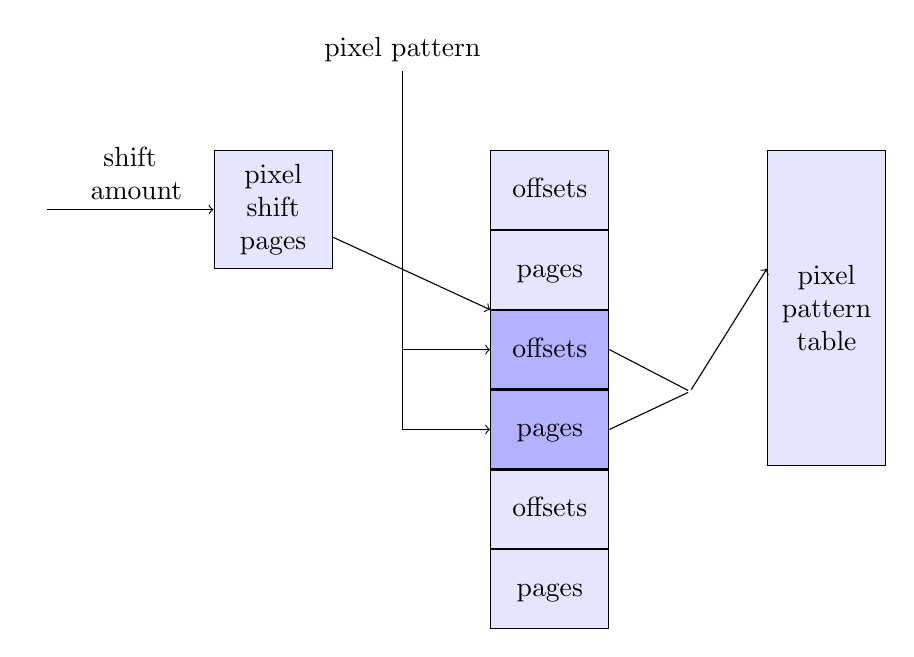
\begin{tikzpicture}
  [basicbox/.style={draw,rectangle,inner sep=0pt,minimum width=1.5cm,minimum height=1.5cm,fill=blue!10},
   pageoffsets/.style={basicbox,minimum height=1cm,text height=1.5ex,text depth=.25ex},
   multilinebox/.style={basicbox,text width=1cm,align=center}]
  \node (pixelshiftpages) at (0,0) [multilinebox] {pixel shift pages};
  \node (start) at (-3,0) {};
  \draw [->] (start) -- (pixelshiftpages) node [above,text width=1cm,align=center,midway] {shift amount};
  \node (offsets0) [pageoffsets,anchor=north,below right=0 and 2 of pixelshiftpages.north east] {offsets};
  \node (pages0) [pageoffsets,below=0 of offsets0.south] {pages};
  \node (offsets1) [pageoffsets,below=0 of pages0.south,fill=blue!30] {offsets};
  \node (pages1) [pageoffsets,below=0 of offsets1.south,fill=blue!30] {pages};
  \node (offsets2) [pageoffsets,below=0 of pages1.south] {offsets};
  \node (pages2) [pageoffsets,below=0 of offsets2.south] {pages};
  \draw [->] (pixelshiftpages) -- (offsets1.north west) {};
  \node (pixelpattern) [above left=1 and 0 of offsets0.north west] {pixel pattern};
  \draw [->] (pixelpattern.south) |- (offsets1.west) {};
  \draw [->] (pixelpattern.south) |- (pages1.west) {};
  \node (patterntable) [multilinebox,minimum height=4cm,text width=1.2cm,anchor=north west,below right=0 and 2 of offsets0.north east] {pixel pattern table};
  \node (join) [inner sep=0pt,below right=0 and 1 of offsets1.south east] {};
  \draw (offsets1.east) -- (join);
  \draw (pages1.east) -- (join);
  \draw [->] (join) -- ([yshift=5mm]patterntable.west);
\end{tikzpicture}
\vspace{1em}

The pixel pattern table is a table of every possible pattern of 7 consecutive pixels
spread out over two bytes. This table is 512 entries, each entry being two bytes.
A naive table would have redundancy. For example the pattern {\Tt{}0000100\nwendquote} starting
at column 0 is exactly the same as the pattern {\Tt{}0001000\nwendquote} starting at column 1.
This table eliminates that redundancy.

\nwenddocs{}\nwbegincode{8}\sublabel{NW1Xx3lK-1W8AJS-2}\nwmargintag{{\nwtagstyle{}\subpageref{NW1Xx3lK-1W8AJS-2}}}\moddef{tables~{\nwtagstyle{}\subpageref{NW1Xx3lK-1W8AJS-1}}}\plusendmoddef\nwstartdeflinemarkup\nwprevnextdefs{NW1Xx3lK-1W8AJS-1}{NW1Xx3lK-1W8AJS-3}\nwenddeflinemarkup
    ORG     $A900
\nwlinkedidentc{PIXEL_PATTERN_TABLE}{NW1Xx3lK-1W8AJS-2}:
    INCLUDE "pixel_pattern_table.asm"
\nwindexdefn{\nwixident{PIXEL{\_}PATTERN{\_}TABLE}}{PIXEL:unPATTERN:unTABLE}{NW1Xx3lK-1W8AJS-2}\eatline
\nwidentdefs{\\{{\nwixident{PIXEL{\_}PATTERN{\_}TABLE}}{PIXEL:unPATTERN:unTABLE}}}\nwendcode{}\nwbegindocs{9}\nwdocspar
Now we just need tables which index into {\Tt{}\nwlinkedidentq{PIXEL{\_}PATTERN{\_}TABLE}{NW1Xx3lK-1W8AJS-2}\nwendquote} for every
7-pixel pattern and shift value. This table works by having the page number
for the shifted pixel pattern at index {\Tt{}shift\ *\ 0x100\ +\ 0x80\ +\ pattern\nwendquote}
and the offset at index {\Tt{}shift\ *\ 0x100\ +\ pattern\nwendquote}.

\nwenddocs{}\nwbegincode{10}\sublabel{NW1Xx3lK-1W8AJS-3}\nwmargintag{{\nwtagstyle{}\subpageref{NW1Xx3lK-1W8AJS-3}}}\moddef{tables~{\nwtagstyle{}\subpageref{NW1Xx3lK-1W8AJS-1}}}\plusendmoddef\nwstartdeflinemarkup\nwprevnextdefs{NW1Xx3lK-1W8AJS-2}{NW1Xx3lK-1W8AJS-4}\nwenddeflinemarkup
    ORG     $A200
\nwlinkedidentc{PIXEL_SHIFT_TABLE}{NW1Xx3lK-1W8AJS-3}:
    INCLUDE "pixel_shift_table.asm"
\nwindexdefn{\nwixident{PIXEL{\_}SHIFT{\_}TABLE}}{PIXEL:unSHIFT:unTABLE}{NW1Xx3lK-1W8AJS-3}\eatline
\nwidentdefs{\\{{\nwixident{PIXEL{\_}SHIFT{\_}TABLE}}{PIXEL:unSHIFT:unTABLE}}}\nwendcode{}\nwbegindocs{11}\nwdocspar
Rather than multiplying the shift value by {\Tt{}0x100\nwendquote}, we instead define
another table which holds the page numbers for the shift tables for each
shift value.

\nwenddocs{}\nwbegincode{12}\sublabel{NW1Xx3lK-1W8AJS-4}\nwmargintag{{\nwtagstyle{}\subpageref{NW1Xx3lK-1W8AJS-4}}}\moddef{tables~{\nwtagstyle{}\subpageref{NW1Xx3lK-1W8AJS-1}}}\plusendmoddef\nwstartdeflinemarkup\nwprevnextdefs{NW1Xx3lK-1W8AJS-3}{NW1Xx3lK-1W8AJS-5}\nwenddeflinemarkup
    ORG     $84C1
\nwlinkedidentc{PIXEL_SHIFT_PAGES}{NW1Xx3lK-1W8AJS-4}:
    HEX     A2 A3 A4 A5 A6 A7 A8
\nwindexdefn{\nwixident{PIXEL{\_}SHIFT{\_}PAGES}}{PIXEL:unSHIFT:unPAGES}{NW1Xx3lK-1W8AJS-4}\eatline
\nwidentdefs{\\{{\nwixident{PIXEL{\_}SHIFT{\_}PAGES}}{PIXEL:unSHIFT:unPAGES}}}\nwendcode{}\nwbegindocs{13}\nwdocspar
So we can get shifted pixels by indexing into all these tables.

Now we can define a routine that will take a sprite number and a pixel shift
amount, and write the shifted pixel data into the {\Tt{}\nwlinkedidentq{BLOCK{\_}DATA}{NW1Xx3lK-10jlgu-1}\nwendquote} area. The
routine first shifts the first byte of the sprite into a two-byte area. Then
it shifts the second byte of the sprite, and combines that two-byte result
with the first. Thus, we shift two bytes of sprite data into a three-byte
result.

\begin{center}
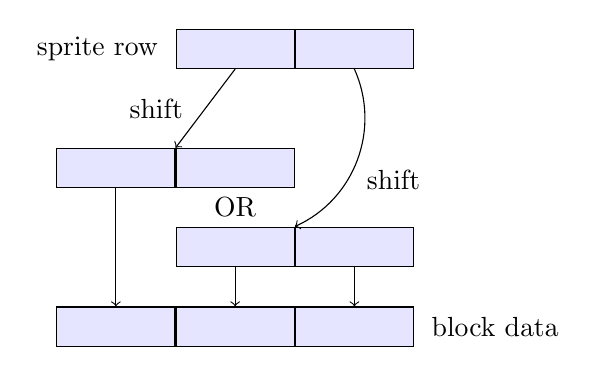
\begin{tikzpicture}
  [basicbox/.style={draw,rectangle,inner sep=0pt,minimum width=1.5cm,minimum height=0.5cm,fill=blue!10}]
  \node (spriterowbyte0) at (0,0) [basicbox] {};
  \node (spriterowbyte1) [basicbox,right=0 of spriterowbyte0.east] {};
  \node (spriterowlabel) [left=0.1 of spriterowbyte0.west] {sprite row};
  \node (shifted0byte0) [basicbox,below left=1 and 0 of spriterowbyte0.south west] {};
  \node (shifted0byte1) [basicbox,right=0 of shifted0byte0.east] {};
  \node (shifted1byte0) [basicbox,below right=2 and 0 of spriterowbyte0.south west] {};
  \node (shifted1byte1) [basicbox,right=0 of shifted1byte0.east] {};
  \node (orlabel) [below=0 of shifted0byte1] {OR};
  \draw [->] (spriterowbyte0.south) -- (shifted0byte0.north east)
    node [left,text width=1cm,align=center,midway] {shift};
  \draw [->] (spriterowbyte1.south) to [auto, bend left=45] node {shift} (shifted1byte0.north east);
  \node (result0) [basicbox,below left=0.5 and 0 of shifted1byte0.south west] {};
  \node (result1) [basicbox,right=0 of result0.east] {};
  \node (result2) [basicbox,right=0 of result1.east] {};
  \draw [->] (shifted0byte0) -- (result0) {};
  \draw [->] (shifted1byte0) -- (result1) {};
  \draw [->] (shifted1byte1) -- (result2) {};
  \node (blocklabel) [right=0.1 of result2.east] {block data};
\end{tikzpicture}
\end{center}

Rather than load addresses from the tables and store them, the routine
modifies its own instructions with those addresses.

\nwenddocs{}\nwbegincode{14}\sublabel{NW1Xx3lK-10jlgu-2}\nwmargintag{{\nwtagstyle{}\subpageref{NW1Xx3lK-10jlgu-2}}}\moddef{defines~{\nwtagstyle{}\subpageref{NW1Xx3lK-10jlgu-1}}}\plusendmoddef\nwstartdeflinemarkup\nwprevnextdefs{NW1Xx3lK-10jlgu-1}{NW1Xx3lK-10jlgu-3}\nwenddeflinemarkup
    ORG     $0A
\nwlinkedidentc{TMP_PTR}{NW1Xx3lK-10jlgu-2}         DS.W    1
    ORG     $1D
\nwlinkedidentc{ROW_COUNT}{NW1Xx3lK-10jlgu-2}       DS      1
\nwlinkedidentc{SPRITE_NUM}{NW1Xx3lK-10jlgu-2}      DS      1
\nwindexdefn{\nwixident{TMP{\_}PTR}}{TMP:unPTR}{NW1Xx3lK-10jlgu-2}\nwindexdefn{\nwixident{ROW{\_}COUNT}}{ROW:unCOUNT}{NW1Xx3lK-10jlgu-2}\nwindexdefn{\nwixident{SPRITE{\_}NUM}}{SPRITE:unNUM}{NW1Xx3lK-10jlgu-2}\eatline
\nwidentdefs{\\{{\nwixident{ROW{\_}COUNT}}{ROW:unCOUNT}}\\{{\nwixident{SPRITE{\_}NUM}}{SPRITE:unNUM}}\\{{\nwixident{TMP{\_}PTR}}{TMP:unPTR}}}\nwendcode{}\nwbegindocs{15}\nwdocspar
\nwenddocs{}\nwbegincode{16}\sublabel{NW1Xx3lK-8jv1b-1}\nwmargintag{{\nwtagstyle{}\subpageref{NW1Xx3lK-8jv1b-1}}}\moddef{routines~{\nwtagstyle{}\subpageref{NW1Xx3lK-8jv1b-1}}}\endmoddef\nwstartdeflinemarkup\nwprevnextdefs{\relax}{NW1Xx3lK-8jv1b-2}\nwenddeflinemarkup
    ORG     $8438
\nwlinkedidentc{COMPUTE_SHIFTED_SPRITE}{NW1Xx3lK-8jv1b-1}:
    SUBROUTINE
    ; Enter routine with X set to pixel shift amount and
    ; \nwlinkedidentc{SPRITE_NUM}{NW1Xx3lK-10jlgu-2} containing the sprite number to read.

.offset_table       EQU $A000               ; Target addresses in read
.page_table         EQU $A080               ; instructions. The only truly
.shift_ptr_byte0    EQU $A000               ; necessary value here is the
.shift_ptr_byte1    EQU $A000               ; 0x80 in .shift_ptr_byte0.

    LDA     #$0B                            ; 11 rows
    STA     \nwlinkedidentc{ROW_COUNT}{NW1Xx3lK-10jlgu-2}
    LDA     #<\nwlinkedidentc{SPRITE_DATA}{NW1Xx3lK-1W8AJS-1}
    STA     \nwlinkedidentc{TMP_PTR}{NW1Xx3lK-10jlgu-2}
    LDA     #>\nwlinkedidentc{SPRITE_DATA}{NW1Xx3lK-1W8AJS-1}
    STA     \nwlinkedidentc{TMP_PTR}{NW1Xx3lK-10jlgu-2}+1                       ; \nwlinkedidentc{TMP_PTR}{NW1Xx3lK-10jlgu-2} = \nwlinkedidentc{SPRITE_DATA}{NW1Xx3lK-1W8AJS-1}
    LDA     \nwlinkedidentc{PIXEL_SHIFT_PAGES}{NW1Xx3lK-1W8AJS-4}, X
    STA     .rd_offset_table + 2
    STA     .rd_page_table + 2
    STA     .rd_offset_table2 + 2
    STA     .rd_page_table2 + 2             ; Fix up pages in lookup instructions
                                            ; based on shift amount (X).

    LDX     #$00                            ; X is the offset into \nwlinkedidentc{BLOCK_DATA}{NW1Xx3lK-10jlgu-1}.

.loop:                                      ; === LOOP === (over all 11 rows)
    LDY     \nwlinkedidentc{SPRITE_NUM}{NW1Xx3lK-10jlgu-2}
    LDA     (\nwlinkedidentc{TMP_PTR}{NW1Xx3lK-10jlgu-2}), Y
    TAY                                     ; Get sprite pixel data.

.rd_offset_table:
    LDA     .offset_table, Y                ; Load offset for shift amount.
    STA     .rd_shift_ptr_byte0 + 1
    CLC
    ADC     #$01
    STA     .rd_shift_ptr_byte1 + 1         ; Fix up instruction offsets with it.
.rd_page_table:
    LDA     .page_table, Y                  ; Load page for shift amount.
    STA     .rd_shift_ptr_byte0 + 2
    STA     .rd_shift_ptr_byte1 + 2         ; Fix up instruction page with it.

.rd_shift_ptr_byte0:
    LDA     .shift_ptr_byte0                ; Read shifted pixel data byte 0
    STA     \nwlinkedidentc{BLOCK_DATA}{NW1Xx3lK-10jlgu-1}, X                   ; and store in block data byte 0.
.rd_shift_ptr_byte1:
    LDA     .shift_ptr_byte1                ; Read shifted pixel data byte 1
    STA     \nwlinkedidentc{BLOCK_DATA}{NW1Xx3lK-10jlgu-1}+1, X                 ; and store in block data byte 1.

    LDA     \nwlinkedidentc{TMP_PTR}{NW1Xx3lK-10jlgu-2}
    CLC
    ADC     #$68
    STA     \nwlinkedidentc{TMP_PTR}{NW1Xx3lK-10jlgu-2}
    LDA     \nwlinkedidentc{TMP_PTR}{NW1Xx3lK-10jlgu-2}+1
    ADC     #$00
    STA     \nwlinkedidentc{TMP_PTR}{NW1Xx3lK-10jlgu-2}+1                       ; \nwlinkedidentc{TMP_PTR}{NW1Xx3lK-10jlgu-2}++

    ; Now basically do the same thing with the second sprite byte

    LDY     \nwlinkedidentc{SPRITE_NUM}{NW1Xx3lK-10jlgu-2}
    LDA     (\nwlinkedidentc{TMP_PTR}{NW1Xx3lK-10jlgu-2}), Y
    TAY                                     ; Get sprite pixel data.

.rd_offset_table2:
    LDA     .offset_table, Y                ; Load offset for shift amount.
    STA     .rd_shift_ptr2_byte0 + 1
    CLC
    ADC     #$01
    STA     .rd_shift_ptr2_byte1 + 1        ; Fix up instruction offsets with it.
.rd_page_table2:
    LDA     .page_table, Y                  ; Load page for shift amount.
    STA     .rd_shift_ptr2_byte0 + 2
    STA     .rd_shift_ptr2_byte1 + 2        ; Fix up instruction page with it.

.rd_shift_ptr2_byte0:
    LDA     .shift_ptr_byte0                ; Read shifted pixel data byte 0
    ORA     \nwlinkedidentc{BLOCK_DATA}{NW1Xx3lK-10jlgu-1}+1, X                 ; OR with previous block data byte 1
    STA     \nwlinkedidentc{BLOCK_DATA}{NW1Xx3lK-10jlgu-1}+1, X                 ; and store in block data byte 1.
.rd_shift_ptr2_byte1:
    LDA     .shift_ptr_byte1                ; Read shifted pixel data byte 1
    STA     \nwlinkedidentc{BLOCK_DATA}{NW1Xx3lK-10jlgu-1}+2, X                 ; and store in block data byte 2.

    LDA     \nwlinkedidentc{TMP_PTR}{NW1Xx3lK-10jlgu-2}
    CLC
    ADC     #$68
    STA     \nwlinkedidentc{TMP_PTR}{NW1Xx3lK-10jlgu-2}
    LDA     \nwlinkedidentc{TMP_PTR}{NW1Xx3lK-10jlgu-2}+1
    ADC     #$00
    STA     \nwlinkedidentc{TMP_PTR}{NW1Xx3lK-10jlgu-2}+1                       ; \nwlinkedidentc{TMP_PTR}{NW1Xx3lK-10jlgu-2}++

    INX
    INX
    INX                                     ; X += 3
    DEC     \nwlinkedidentc{ROW_COUNT}{NW1Xx3lK-10jlgu-2}                       ; \nwlinkedidentc{ROW_COUNT}{NW1Xx3lK-10jlgu-2}--
    BNE     .loop                           ; loop while \nwlinkedidentc{ROW_COUNT}{NW1Xx3lK-10jlgu-2} > 0
    RTS
\nwindexdefn{\nwixident{COMPUTE{\_}SHIFTED{\_}SPRITE}}{COMPUTE:unSHIFTED:unSPRITE}{NW1Xx3lK-8jv1b-1}\eatline
\nwalsodefined{\\{NW1Xx3lK-8jv1b-2}\\{NW1Xx3lK-8jv1b-3}\\{NW1Xx3lK-8jv1b-4}}\nwnotused{routines}\nwidentdefs{\\{{\nwixident{COMPUTE{\_}SHIFTED{\_}SPRITE}}{COMPUTE:unSHIFTED:unSPRITE}}}\nwidentuses{\\{{\nwixident{BLOCK{\_}DATA}}{BLOCK:unDATA}}\\{{\nwixident{PIXEL{\_}SHIFT{\_}PAGES}}{PIXEL:unSHIFT:unPAGES}}\\{{\nwixident{ROW{\_}COUNT}}{ROW:unCOUNT}}\\{{\nwixident{SPRITE{\_}DATA}}{SPRITE:unDATA}}\\{{\nwixident{SPRITE{\_}NUM}}{SPRITE:unNUM}}\\{{\nwixident{TMP{\_}PTR}}{TMP:unPTR}}}\nwindexuse{\nwixident{BLOCK{\_}DATA}}{BLOCK:unDATA}{NW1Xx3lK-8jv1b-1}\nwindexuse{\nwixident{PIXEL{\_}SHIFT{\_}PAGES}}{PIXEL:unSHIFT:unPAGES}{NW1Xx3lK-8jv1b-1}\nwindexuse{\nwixident{ROW{\_}COUNT}}{ROW:unCOUNT}{NW1Xx3lK-8jv1b-1}\nwindexuse{\nwixident{SPRITE{\_}DATA}}{SPRITE:unDATA}{NW1Xx3lK-8jv1b-1}\nwindexuse{\nwixident{SPRITE{\_}NUM}}{SPRITE:unNUM}{NW1Xx3lK-8jv1b-1}\nwindexuse{\nwixident{TMP{\_}PTR}}{TMP:unPTR}{NW1Xx3lK-8jv1b-1}\nwendcode{}\nwbegindocs{17}\nwdocspar
\section{Memory mapped graphics}

The Apple II maps the area from {\Tt{}{\$}2000-{\$}3FFF\nwendquote} to high-res graphics page 1 (HGR1),
and {\Tt{}{\$}4000-{\$}5FFF\nwendquote} to page 2 (HGR2). Within a row, consecutive bytes map to
consecutive pixels. However, rows themselves are not consecutive in memory.

To make it easy to convert a row number from 0 to 191 to a base address, Lode Runner has
a table and a routine to use that table.

\nwenddocs{}\nwbegincode{18}\sublabel{NW1Xx3lK-1W8AJS-5}\nwmargintag{{\nwtagstyle{}\subpageref{NW1Xx3lK-1W8AJS-5}}}\moddef{tables~{\nwtagstyle{}\subpageref{NW1Xx3lK-1W8AJS-1}}}\plusendmoddef\nwstartdeflinemarkup\nwprevnextdefs{NW1Xx3lK-1W8AJS-4}{NW1Xx3lK-1W8AJS-6}\nwenddeflinemarkup
    ORG     $1A85
\nwlinkedidentc{ROW_TO_OFFSET_LO}{NW1Xx3lK-1W8AJS-5}:
    INCLUDE "row_to_offset_lo_table.asm"
\nwlinkedidentc{ROW_TO_OFFSET_HI}{NW1Xx3lK-1W8AJS-5}:
    INCLUDE "row_to_offset_hi_table.asm"
\nwindexdefn{\nwixident{ROW{\_}TO{\_}OFFSET{\_}LO}}{ROW:unTO:unOFFSET:unLO}{NW1Xx3lK-1W8AJS-5}\nwindexdefn{\nwixident{ROW{\_}TO{\_}OFFSET{\_}HI}}{ROW:unTO:unOFFSET:unHI}{NW1Xx3lK-1W8AJS-5}\eatline
\nwidentdefs{\\{{\nwixident{ROW{\_}TO{\_}OFFSET{\_}HI}}{ROW:unTO:unOFFSET:unHI}}\\{{\nwixident{ROW{\_}TO{\_}OFFSET{\_}LO}}{ROW:unTO:unOFFSET:unLO}}}\nwendcode{}\nwbegindocs{19}\nwdocspar
\nwenddocs{}\nwbegincode{20}\sublabel{NW1Xx3lK-10jlgu-3}\nwmargintag{{\nwtagstyle{}\subpageref{NW1Xx3lK-10jlgu-3}}}\moddef{defines~{\nwtagstyle{}\subpageref{NW1Xx3lK-10jlgu-1}}}\plusendmoddef\nwstartdeflinemarkup\nwprevnextdefs{NW1Xx3lK-10jlgu-2}{NW1Xx3lK-10jlgu-4}\nwenddeflinemarkup
    ORG     $0C
\nwlinkedidentc{ROW_ADDR}{NW1Xx3lK-10jlgu-3}    DS      2
    ORG     $1F
\nwlinkedidentc{HGR_PAGE}{NW1Xx3lK-10jlgu-3}    DS      1       ; 0x20 for HGR1, 0x40 for HGR2
\nwindexdefn{\nwixident{ROW{\_}ADDR}}{ROW:unADDR}{NW1Xx3lK-10jlgu-3}\nwindexdefn{\nwixident{HGR{\_}PAGE}}{HGR:unPAGE}{NW1Xx3lK-10jlgu-3}\eatline
\nwidentdefs{\\{{\nwixident{HGR{\_}PAGE}}{HGR:unPAGE}}\\{{\nwixident{ROW{\_}ADDR}}{ROW:unADDR}}}\nwendcode{}\nwbegindocs{21}\nwdocspar
\nwenddocs{}\nwbegincode{22}\sublabel{NW1Xx3lK-8jv1b-2}\nwmargintag{{\nwtagstyle{}\subpageref{NW1Xx3lK-8jv1b-2}}}\moddef{routines~{\nwtagstyle{}\subpageref{NW1Xx3lK-8jv1b-1}}}\plusendmoddef\nwstartdeflinemarkup\nwprevnextdefs{NW1Xx3lK-8jv1b-1}{NW1Xx3lK-8jv1b-3}\nwenddeflinemarkup
    ORG     $7A31
\nwlinkedidentc{ROW_TO_ADDR}{NW1Xx3lK-8jv1b-2}:
    SUBROUTINE
    ; Enter routine with Y set to row. Base address
    ; (for column 0) will be placed in \nwlinkedidentc{ROW_ADDR}{NW1Xx3lK-10jlgu-3}.

    LDA     \nwlinkedidentc{ROW_TO_OFFSET_LO}{NW1Xx3lK-1W8AJS-5}, Y
    STA     \nwlinkedidentc{ROW_ADDR}{NW1Xx3lK-10jlgu-3}
    LDA     \nwlinkedidentc{ROW_TO_OFFSET_HI}{NW1Xx3lK-1W8AJS-5}, Y
    ORA     \nwlinkedidentc{HGR_PAGE}{NW1Xx3lK-10jlgu-3}
    STA     \nwlinkedidentc{ROW_ADDR}{NW1Xx3lK-10jlgu-3}+1
    RTS
\nwindexdefn{\nwixident{ROW{\_}TO{\_}ADDR}}{ROW:unTO:unADDR}{NW1Xx3lK-8jv1b-2}\eatline
\nwidentdefs{\\{{\nwixident{ROW{\_}TO{\_}ADDR}}{ROW:unTO:unADDR}}}\nwidentuses{\\{{\nwixident{HGR{\_}PAGE}}{HGR:unPAGE}}\\{{\nwixident{ROW{\_}ADDR}}{ROW:unADDR}}\\{{\nwixident{ROW{\_}TO{\_}OFFSET{\_}HI}}{ROW:unTO:unOFFSET:unHI}}\\{{\nwixident{ROW{\_}TO{\_}OFFSET{\_}LO}}{ROW:unTO:unOFFSET:unLO}}}\nwindexuse{\nwixident{HGR{\_}PAGE}}{HGR:unPAGE}{NW1Xx3lK-8jv1b-2}\nwindexuse{\nwixident{ROW{\_}ADDR}}{ROW:unADDR}{NW1Xx3lK-8jv1b-2}\nwindexuse{\nwixident{ROW{\_}TO{\_}OFFSET{\_}HI}}{ROW:unTO:unOFFSET:unHI}{NW1Xx3lK-8jv1b-2}\nwindexuse{\nwixident{ROW{\_}TO{\_}OFFSET{\_}LO}}{ROW:unTO:unOFFSET:unLO}{NW1Xx3lK-8jv1b-2}\nwendcode{}\nwbegindocs{23}\nwdocspar
Lode Runner's screens are organized into 28 sprites across by 17 sprites
down. To convert between sprite coordinates and screen coordinates, we
use tables and lookup routines. Each sprite is 10 pixels across by 11 pixels down.

\nwenddocs{}\nwbegincode{24}\sublabel{NW1Xx3lK-1W8AJS-6}\nwmargintag{{\nwtagstyle{}\subpageref{NW1Xx3lK-1W8AJS-6}}}\moddef{tables~{\nwtagstyle{}\subpageref{NW1Xx3lK-1W8AJS-1}}}\plusendmoddef\nwstartdeflinemarkup\nwprevnextdefs{NW1Xx3lK-1W8AJS-5}{NW1Xx3lK-1W8AJS-7}\nwenddeflinemarkup
    ORG     $1C35
\nwlinkedidentc{ROW_TABLE2}{NW1Xx3lK-1W8AJS-6}:
    ; 28 rows of 5 pixels each
    HEX     00 05 0a 0f 14 19 1e 23 28 2d 32 37 3c 41 46 4b
    HEX     50 55 5a 5f 64 69 6e 73 78 7d 82 87
\nwlinkedidentc{ROW_TABLE}{NW1Xx3lK-1W8AJS-6}:
    ; 17 rows of 11 pixels each
    HEX     00 0B 16 21 2C 37 42 4D 58 63 6E 79 84 8F 9A A5
    HEX     B5
\nwlinkedidentc{COL_TABLE}{NW1Xx3lK-1W8AJS-6}:
    ; Byte number
    HEX     00 01 02 04 05 07 08 0A 0B 0C 0E 0F 11 12 14 15
    HEX     16 18 19 1B 1C 1E 1F 20 22 23 25 26
\nwlinkedidentc{COL_SHIFT_TABLE}{NW1Xx3lK-1W8AJS-6}:
    ; Right shift amount
    HEX     00 03 06 02 05 01 04 00 03 06 02 05 01 04 00 03
    HEX     06 02 05 01 04 00 03 06 02 05 01 04
\nwindexdefn{\nwixident{ROW{\_}TABLE}}{ROW:unTABLE}{NW1Xx3lK-1W8AJS-6}\nwindexdefn{\nwixident{COL{\_}TABLE}}{COL:unTABLE}{NW1Xx3lK-1W8AJS-6}\nwindexdefn{\nwixident{ROW{\_}TABLE2}}{ROW:unTABLE2}{NW1Xx3lK-1W8AJS-6}\nwindexdefn{\nwixident{COL{\_}SHIFT{\_}TABLE}}{COL:unSHIFT:unTABLE}{NW1Xx3lK-1W8AJS-6}\eatline
\nwidentdefs{\\{{\nwixident{COL{\_}SHIFT{\_}TABLE}}{COL:unSHIFT:unTABLE}}\\{{\nwixident{COL{\_}TABLE}}{COL:unTABLE}}\\{{\nwixident{ROW{\_}TABLE}}{ROW:unTABLE}}\\{{\nwixident{ROW{\_}TABLE2}}{ROW:unTABLE2}}}\nwendcode{}\nwbegindocs{25}\nwdocspar
\nwenddocs{}\nwbegincode{26}\sublabel{NW1Xx3lK-8jv1b-3}\nwmargintag{{\nwtagstyle{}\subpageref{NW1Xx3lK-8jv1b-3}}}\moddef{routines~{\nwtagstyle{}\subpageref{NW1Xx3lK-8jv1b-1}}}\plusendmoddef\nwstartdeflinemarkup\nwprevnextdefs{NW1Xx3lK-8jv1b-2}{NW1Xx3lK-8jv1b-4}\nwenddeflinemarkup
    ORG     $885D
\nwlinkedidentc{GET_ROWNUM_FOR}{NW1Xx3lK-8jv1b-3}:
    SUBROUTINE
    ; Enter routine with Y set to sprite row. On
    ; return, Y will be set to screen row.
    ; We can also set X to something, and on return
    ; X is set to something based on \nwlinkedidentc{ROW_TABLE2}{NW1Xx3lK-1W8AJS-6}, but
    ; so far I'm not sure what it's used for.

    LDA     \nwlinkedidentc{ROW_TABLE}{NW1Xx3lK-1W8AJS-6}, Y
    PHA
    LDA     \nwlinkedidentc{ROW_TABLE2}{NW1Xx3lK-1W8AJS-6}, X
    TAX                         ; X = \nwlinkedidentc{ROW_TABLE2}{NW1Xx3lK-1W8AJS-6}[X]
    PLA
    TAY                         ; Y = \nwlinkedidentc{ROW_TABLE}{NW1Xx3lK-1W8AJS-6}[Y]
    RTS

\nwlinkedidentc{GET_COLNUM_FOR}{NW1Xx3lK-8jv1b-3}:
    SUBROUTINE
    ; Enter routine with X set to sprite number. On
    ; return, A will be set to screen column byte number
    ; and X will be set to an additional right shift amount.

    LDA     \nwlinkedidentc{COL_TABLE}{NW1Xx3lK-1W8AJS-6}, X
    PHA                         ; A = COL_TABLE2[X]
    LDA     \nwlinkedidentc{COL_SHIFT_TABLE}{NW1Xx3lK-1W8AJS-6}, X
    TAX                         ; X = \nwlinkedidentc{COL_SHIFT_TABLE}{NW1Xx3lK-1W8AJS-6}[X]
    PLA
    RTS
\nwindexdefn{\nwixident{GET{\_}ROWNUM{\_}FOR}}{GET:unROWNUM:unFOR}{NW1Xx3lK-8jv1b-3}\nwindexdefn{\nwixident{GET{\_}COLNUM{\_}FOR}}{GET:unCOLNUM:unFOR}{NW1Xx3lK-8jv1b-3}\eatline
\nwidentdefs{\\{{\nwixident{GET{\_}COLNUM{\_}FOR}}{GET:unCOLNUM:unFOR}}\\{{\nwixident{GET{\_}ROWNUM{\_}FOR}}{GET:unROWNUM:unFOR}}}\nwidentuses{\\{{\nwixident{COL{\_}SHIFT{\_}TABLE}}{COL:unSHIFT:unTABLE}}\\{{\nwixident{COL{\_}TABLE}}{COL:unTABLE}}\\{{\nwixident{ROW{\_}TABLE}}{ROW:unTABLE}}\\{{\nwixident{ROW{\_}TABLE2}}{ROW:unTABLE2}}}\nwindexuse{\nwixident{COL{\_}SHIFT{\_}TABLE}}{COL:unSHIFT:unTABLE}{NW1Xx3lK-8jv1b-3}\nwindexuse{\nwixident{COL{\_}TABLE}}{COL:unTABLE}{NW1Xx3lK-8jv1b-3}\nwindexuse{\nwixident{ROW{\_}TABLE}}{ROW:unTABLE}{NW1Xx3lK-8jv1b-3}\nwindexuse{\nwixident{ROW{\_}TABLE2}}{ROW:unTABLE2}{NW1Xx3lK-8jv1b-3}\nwendcode{}\nwbegindocs{27}\nwdocspar
Now we can finally write the routines that draw a sprite on the screen.
There are two entry points, one to draw on HGR1, and one for HGR2.

\nwenddocs{}\nwbegincode{28}\sublabel{NW1Xx3lK-10jlgu-4}\nwmargintag{{\nwtagstyle{}\subpageref{NW1Xx3lK-10jlgu-4}}}\moddef{defines~{\nwtagstyle{}\subpageref{NW1Xx3lK-10jlgu-1}}}\plusendmoddef\nwstartdeflinemarkup\nwprevnextdefs{NW1Xx3lK-10jlgu-3}{\relax}\nwenddeflinemarkup
    ORG     $1B
\nwlinkedidentc{ROWNUM}{NW1Xx3lK-10jlgu-4}          DS      1
\nwlinkedidentc{COLNUM}{NW1Xx3lK-10jlgu-4}          DS      1
    ORG     $50
MASK0           DS      1
MASK1           DS      1
    ORG     $71
\nwlinkedidentc{COL_SHIFT_AMT}{NW1Xx3lK-10jlgu-4}   DS      1
    ORG     $85
\nwlinkedidentc{GAME_COLNUM}{NW1Xx3lK-10jlgu-4}     DS      1
\nwlinkedidentc{GAME_ROWNUM}{NW1Xx3lK-10jlgu-4}     DS      1
\nwindexdefn{\nwixident{ROWNUM}}{ROWNUM}{NW1Xx3lK-10jlgu-4}\nwindexdefn{\nwixident{COLNUM}}{COLNUM}{NW1Xx3lK-10jlgu-4}\nwindexdefn{\nwixident{COL{\_}SHIFT{\_}AMT}}{COL:unSHIFT:unAMT}{NW1Xx3lK-10jlgu-4}\nwindexdefn{\nwixident{GAME{\_}COLNUM}}{GAME:unCOLNUM}{NW1Xx3lK-10jlgu-4}\nwindexdefn{\nwixident{GAME{\_}ROWNUM}}{GAME:unROWNUM}{NW1Xx3lK-10jlgu-4}\eatline
\nwidentdefs{\\{{\nwixident{COL{\_}SHIFT{\_}AMT}}{COL:unSHIFT:unAMT}}\\{{\nwixident{COLNUM}}{COLNUM}}\\{{\nwixident{GAME{\_}COLNUM}}{GAME:unCOLNUM}}\\{{\nwixident{GAME{\_}ROWNUM}}{GAME:unROWNUM}}\\{{\nwixident{ROWNUM}}{ROWNUM}}}\nwendcode{}\nwbegindocs{29}\nwdocspar
\nwenddocs{}\nwbegincode{30}\sublabel{NW1Xx3lK-1W8AJS-7}\nwmargintag{{\nwtagstyle{}\subpageref{NW1Xx3lK-1W8AJS-7}}}\moddef{tables~{\nwtagstyle{}\subpageref{NW1Xx3lK-1W8AJS-1}}}\plusendmoddef\nwstartdeflinemarkup\nwprevnextdefs{NW1Xx3lK-1W8AJS-6}{\relax}\nwenddeflinemarkup
    ORG     $8328
\nwlinkedidentc{PIXEL_MASK0}{NW1Xx3lK-1W8AJS-7}:
    BYTE    %00000000
    BYTE    %00000001
    BYTE    %00000011
    BYTE    %00000111
    BYTE    %00001111
    BYTE    %00011111
    BYTE    %00111111
\nwlinkedidentc{PIXEL_MASK1}{NW1Xx3lK-1W8AJS-7}:
    BYTE    %11111000
    BYTE    %11110000
    BYTE    %11100000
    BYTE    %11000000
    BYTE    %10000000
    BYTE    %11111110
    BYTE    %11111100
\nwindexdefn{\nwixident{PIXEL{\_}MASK0}}{PIXEL:unMASK0}{NW1Xx3lK-1W8AJS-7}\nwindexdefn{\nwixident{PIXEL{\_}MASK1}}{PIXEL:unMASK1}{NW1Xx3lK-1W8AJS-7}\eatline
\nwidentdefs{\\{{\nwixident{PIXEL{\_}MASK0}}{PIXEL:unMASK0}}\\{{\nwixident{PIXEL{\_}MASK1}}{PIXEL:unMASK1}}}\nwendcode{}\nwbegindocs{31}\nwdocspar
\nwenddocs{}\nwbegincode{32}\sublabel{NW1Xx3lK-8jv1b-4}\nwmargintag{{\nwtagstyle{}\subpageref{NW1Xx3lK-8jv1b-4}}}\moddef{routines~{\nwtagstyle{}\subpageref{NW1Xx3lK-8jv1b-1}}}\plusendmoddef\nwstartdeflinemarkup\nwprevnextdefs{NW1Xx3lK-8jv1b-3}{\relax}\nwenddeflinemarkup
    ORG     $82AA
\nwlinkedidentc{DRAW_SPRITE_PAGE1}{NW1Xx3lK-8jv1b-4}:
    SUBROUTINE
    ; Enter routine with A set to sprite number to draw,
    ; \nwlinkedidentc{GAME_ROWNUM}{NW1Xx3lK-10jlgu-4} set to the row to draw it at, and \nwlinkedidentc{GAME_COLNUM}{NW1Xx3lK-10jlgu-4}
    ; set to the column to draw it at.

    STA     \nwlinkedidentc{SPRITE_NUM}{NW1Xx3lK-10jlgu-2}
    LDA     #$20                ; Page number for HGR1
    BNE     DRAW_SPRITE         ; Actually unconditional jump

\nwlinkedidentc{DRAW_SPRITE_PAGE2}{NW1Xx3lK-8jv1b-4}:
    SUBROUTINE
    ; Enter routine with A set to sprite number to draw,
    ; \nwlinkedidentc{GAME_ROWNUM}{NW1Xx3lK-10jlgu-4} set to the row to draw it at, and \nwlinkedidentc{GAME_COLNUM}{NW1Xx3lK-10jlgu-4}
    ; set to the column to draw it at.

    STA     \nwlinkedidentc{SPRITE_NUM}{NW1Xx3lK-10jlgu-2}
    LDA     #$40                ; Page number for HGR2
    ; fallthrough

DRAW_SPRITE:
    STA     \nwlinkedidentc{HGR_PAGE}{NW1Xx3lK-10jlgu-3}
    LDY     \nwlinkedidentc{GAME_ROWNUM}{NW1Xx3lK-10jlgu-4}
    JSR     \nwlinkedidentc{GET_ROWNUM_FOR}{NW1Xx3lK-8jv1b-3}
    STY     \nwlinkedidentc{ROWNUM}{NW1Xx3lK-10jlgu-4}              ; \nwlinkedidentc{ROWNUM}{NW1Xx3lK-10jlgu-4} = \nwlinkedidentc{ROW_TABLE}{NW1Xx3lK-1W8AJS-6}[\nwlinkedidentc{GAME_ROWNUM}{NW1Xx3lK-10jlgu-4}]

    LDX     \nwlinkedidentc{GAME_COLNUM}{NW1Xx3lK-10jlgu-4}
    JSR     \nwlinkedidentc{GET_COLNUM_FOR}{NW1Xx3lK-8jv1b-3}
    STA     \nwlinkedidentc{COLNUM}{NW1Xx3lK-10jlgu-4}              ; \nwlinkedidentc{COLNUM}{NW1Xx3lK-10jlgu-4} = \nwlinkedidentc{COL_TABLE}{NW1Xx3lK-1W8AJS-6}[\nwlinkedidentc{GAME_COLNUM}{NW1Xx3lK-10jlgu-4}]
    STX     \nwlinkedidentc{COL_SHIFT_AMT}{NW1Xx3lK-10jlgu-4}       ; \nwlinkedidentc{COL_SHIFT_AMT}{NW1Xx3lK-10jlgu-4} = \nwlinkedidentc{COL_SHIFT_TABLE}{NW1Xx3lK-1W8AJS-6}[\nwlinkedidentc{GAME_COLNUM}{NW1Xx3lK-10jlgu-4}]

    LDA     \nwlinkedidentc{PIXEL_MASK0}{NW1Xx3lK-1W8AJS-7}, X
    STA     MASK0               ; MASK0 = \nwlinkedidentc{PIXEL_MASK0}{NW1Xx3lK-1W8AJS-7}[\nwlinkedidentc{COL_SHIFT_AMT}{NW1Xx3lK-10jlgu-4}]
    LDA     \nwlinkedidentc{PIXEL_MASK1}{NW1Xx3lK-1W8AJS-7}, X
    STA     MASK1               ; MASK1 = \nwlinkedidentc{PIXEL_MASK1}{NW1Xx3lK-1W8AJS-7}[\nwlinkedidentc{COL_SHIFT_AMT}{NW1Xx3lK-10jlgu-4}]

    JSR     \nwlinkedidentc{COMPUTE_SHIFTED_SPRITE}{NW1Xx3lK-8jv1b-1}

    LDA     #$0B
    STA     \nwlinkedidentc{ROW_COUNT}{NW1Xx3lK-10jlgu-2}
    LDX     #$00
    LDA     \nwlinkedidentc{COL_SHIFT_AMT}{NW1Xx3lK-10jlgu-4}
    CMP     #$05
    BCS     .need_3_bytes       ; if \nwlinkedidentc{COL_SHIFT_AMT}{NW1Xx3lK-10jlgu-4} >= 5, we need to alter three screen bytes.

.loop1:
    LDY     \nwlinkedidentc{ROWNUM}{NW1Xx3lK-10jlgu-4}
    JSR     \nwlinkedidentc{ROW_TO_ADDR}{NW1Xx3lK-8jv1b-2}
    LDY     \nwlinkedidentc{COLNUM}{NW1Xx3lK-10jlgu-4}
    LDA     (\nwlinkedidentc{ROW_ADDR}{NW1Xx3lK-10jlgu-3}), Y
    AND     MASK0
    ORA     \nwlinkedidentc{BLOCK_DATA}{NW1Xx3lK-10jlgu-1}, X
    STA     (\nwlinkedidentc{ROW_ADDR}{NW1Xx3lK-10jlgu-3}), Y       ; screen[\nwlinkedidentc{COLNUM}{NW1Xx3lK-10jlgu-4}] = screen[\nwlinkedidentc{COLNUM}{NW1Xx3lK-10jlgu-4}] & MASK0 | \nwlinkedidentc{BLOCK_DATA}{NW1Xx3lK-10jlgu-1}[X]

    INX                         ; X++
    INY                         ; Y++
    LDA     (\nwlinkedidentc{ROW_ADDR}{NW1Xx3lK-10jlgu-3}), Y
    AND     MASK1
    ORA     \nwlinkedidentc{BLOCK_DATA}{NW1Xx3lK-10jlgu-1}+1, X
    STA     (\nwlinkedidentc{ROW_ADDR}{NW1Xx3lK-10jlgu-3}), Y       ; screen[\nwlinkedidentc{COLNUM}{NW1Xx3lK-10jlgu-4}+1] = screen[\nwlinkedidentc{COLNUM}{NW1Xx3lK-10jlgu-4}+1] & MASK1 | \nwlinkedidentc{BLOCK_DATA}{NW1Xx3lK-10jlgu-1}[X+1]

    INX
    INX                         ; X += 2
    INC     \nwlinkedidentc{ROWNUM}{NW1Xx3lK-10jlgu-4}              ; \nwlinkedidentc{ROWNUM}{NW1Xx3lK-10jlgu-4}++
    DEC     \nwlinkedidentc{ROW_COUNT}{NW1Xx3lK-10jlgu-2}           ; \nwlinkedidentc{ROW_COUNT}{NW1Xx3lK-10jlgu-2}--
    BNE     .loop1              ; loop while \nwlinkedidentc{ROW_COUNT}{NW1Xx3lK-10jlgu-2} > 0
    RTS

.need_3_bytes



\nwindexdefn{\nwixident{DRAW{\_}SPRITE{\_}PAGE1}}{DRAW:unSPRITE:unPAGE1}{NW1Xx3lK-8jv1b-4}\nwindexdefn{\nwixident{DRAW{\_}SPRITE{\_}PAGE2}}{DRAW:unSPRITE:unPAGE2}{NW1Xx3lK-8jv1b-4}\eatline
\nwidentdefs{\\{{\nwixident{DRAW{\_}SPRITE{\_}PAGE1}}{DRAW:unSPRITE:unPAGE1}}\\{{\nwixident{DRAW{\_}SPRITE{\_}PAGE2}}{DRAW:unSPRITE:unPAGE2}}}\nwidentuses{\\{{\nwixident{BLOCK{\_}DATA}}{BLOCK:unDATA}}\\{{\nwixident{COL{\_}SHIFT{\_}AMT}}{COL:unSHIFT:unAMT}}\\{{\nwixident{COL{\_}SHIFT{\_}TABLE}}{COL:unSHIFT:unTABLE}}\\{{\nwixident{COL{\_}TABLE}}{COL:unTABLE}}\\{{\nwixident{COLNUM}}{COLNUM}}\\{{\nwixident{COMPUTE{\_}SHIFTED{\_}SPRITE}}{COMPUTE:unSHIFTED:unSPRITE}}\\{{\nwixident{GAME{\_}COLNUM}}{GAME:unCOLNUM}}\\{{\nwixident{GAME{\_}ROWNUM}}{GAME:unROWNUM}}\\{{\nwixident{GET{\_}COLNUM{\_}FOR}}{GET:unCOLNUM:unFOR}}\\{{\nwixident{GET{\_}ROWNUM{\_}FOR}}{GET:unROWNUM:unFOR}}\\{{\nwixident{HGR{\_}PAGE}}{HGR:unPAGE}}\\{{\nwixident{PIXEL{\_}MASK0}}{PIXEL:unMASK0}}\\{{\nwixident{PIXEL{\_}MASK1}}{PIXEL:unMASK1}}\\{{\nwixident{ROW{\_}ADDR}}{ROW:unADDR}}\\{{\nwixident{ROW{\_}COUNT}}{ROW:unCOUNT}}\\{{\nwixident{ROW{\_}TABLE}}{ROW:unTABLE}}\\{{\nwixident{ROW{\_}TO{\_}ADDR}}{ROW:unTO:unADDR}}\\{{\nwixident{ROWNUM}}{ROWNUM}}\\{{\nwixident{SPRITE{\_}NUM}}{SPRITE:unNUM}}}\nwindexuse{\nwixident{BLOCK{\_}DATA}}{BLOCK:unDATA}{NW1Xx3lK-8jv1b-4}\nwindexuse{\nwixident{COL{\_}SHIFT{\_}AMT}}{COL:unSHIFT:unAMT}{NW1Xx3lK-8jv1b-4}\nwindexuse{\nwixident{COL{\_}SHIFT{\_}TABLE}}{COL:unSHIFT:unTABLE}{NW1Xx3lK-8jv1b-4}\nwindexuse{\nwixident{COL{\_}TABLE}}{COL:unTABLE}{NW1Xx3lK-8jv1b-4}\nwindexuse{\nwixident{COLNUM}}{COLNUM}{NW1Xx3lK-8jv1b-4}\nwindexuse{\nwixident{COMPUTE{\_}SHIFTED{\_}SPRITE}}{COMPUTE:unSHIFTED:unSPRITE}{NW1Xx3lK-8jv1b-4}\nwindexuse{\nwixident{GAME{\_}COLNUM}}{GAME:unCOLNUM}{NW1Xx3lK-8jv1b-4}\nwindexuse{\nwixident{GAME{\_}ROWNUM}}{GAME:unROWNUM}{NW1Xx3lK-8jv1b-4}\nwindexuse{\nwixident{GET{\_}COLNUM{\_}FOR}}{GET:unCOLNUM:unFOR}{NW1Xx3lK-8jv1b-4}\nwindexuse{\nwixident{GET{\_}ROWNUM{\_}FOR}}{GET:unROWNUM:unFOR}{NW1Xx3lK-8jv1b-4}\nwindexuse{\nwixident{HGR{\_}PAGE}}{HGR:unPAGE}{NW1Xx3lK-8jv1b-4}\nwindexuse{\nwixident{PIXEL{\_}MASK0}}{PIXEL:unMASK0}{NW1Xx3lK-8jv1b-4}\nwindexuse{\nwixident{PIXEL{\_}MASK1}}{PIXEL:unMASK1}{NW1Xx3lK-8jv1b-4}\nwindexuse{\nwixident{ROW{\_}ADDR}}{ROW:unADDR}{NW1Xx3lK-8jv1b-4}\nwindexuse{\nwixident{ROW{\_}COUNT}}{ROW:unCOUNT}{NW1Xx3lK-8jv1b-4}\nwindexuse{\nwixident{ROW{\_}TABLE}}{ROW:unTABLE}{NW1Xx3lK-8jv1b-4}\nwindexuse{\nwixident{ROW{\_}TO{\_}ADDR}}{ROW:unTO:unADDR}{NW1Xx3lK-8jv1b-4}\nwindexuse{\nwixident{ROWNUM}}{ROWNUM}{NW1Xx3lK-8jv1b-4}\nwindexuse{\nwixident{SPRITE{\_}NUM}}{SPRITE:unNUM}{NW1Xx3lK-8jv1b-4}\nwendcode{}\nwbegindocs{33}\nwdocspar
\chapter{The whole thing}
We then put together the entire assembly file:

\nwenddocs{}\nwbegincode{34}\sublabel{NW1Xx3lK-1p0Y9w-1}\nwmargintag{{\nwtagstyle{}\subpageref{NW1Xx3lK-1p0Y9w-1}}}\moddef{*~{\nwtagstyle{}\subpageref{NW1Xx3lK-1p0Y9w-1}}}\endmoddef\nwstartdeflinemarkup\nwenddeflinemarkup
\LA{}preamble~{\nwtagstyle{}\subpageref{NW1Xx3lK-1jwKhK-1}}\RA{}
\nwnotused{*}\nwendcode{}\nwbegindocs{35}\nwdocspar

\chapter{Defined Chunks}\par\noindent
\nowebchunks
\chapter{Index}\par\noindent
\nowebindex
\nwenddocs{}

\nwixlogsorted{c}{{*}{NW1Xx3lK-1p0Y9w-1}{\nwixd{NW1Xx3lK-1p0Y9w-1}}}%
\nwixlogsorted{c}{{defines}{NW1Xx3lK-10jlgu-1}{\nwixd{NW1Xx3lK-10jlgu-1}\nwixd{NW1Xx3lK-10jlgu-2}\nwixd{NW1Xx3lK-10jlgu-3}\nwixd{NW1Xx3lK-10jlgu-4}}}%
\nwixlogsorted{c}{{preamble}{NW1Xx3lK-1jwKhK-1}{\nwixd{NW1Xx3lK-1jwKhK-1}\nwixu{NW1Xx3lK-1p0Y9w-1}}}%
\nwixlogsorted{c}{{routines}{NW1Xx3lK-8jv1b-1}{\nwixd{NW1Xx3lK-8jv1b-1}\nwixd{NW1Xx3lK-8jv1b-2}\nwixd{NW1Xx3lK-8jv1b-3}\nwixd{NW1Xx3lK-8jv1b-4}}}%
\nwixlogsorted{c}{{tables}{NW1Xx3lK-1W8AJS-1}{\nwixd{NW1Xx3lK-1W8AJS-1}\nwixd{NW1Xx3lK-1W8AJS-2}\nwixd{NW1Xx3lK-1W8AJS-3}\nwixd{NW1Xx3lK-1W8AJS-4}\nwixd{NW1Xx3lK-1W8AJS-5}\nwixd{NW1Xx3lK-1W8AJS-6}\nwixd{NW1Xx3lK-1W8AJS-7}}}%
\nwixlogsorted{i}{{\nwixident{BLOCK{\_}DATA}}{BLOCK:unDATA}}%
\nwixlogsorted{i}{{\nwixident{COL{\_}SHIFT{\_}AMT}}{COL:unSHIFT:unAMT}}%
\nwixlogsorted{i}{{\nwixident{COL{\_}SHIFT{\_}TABLE}}{COL:unSHIFT:unTABLE}}%
\nwixlogsorted{i}{{\nwixident{COL{\_}TABLE}}{COL:unTABLE}}%
\nwixlogsorted{i}{{\nwixident{COLNUM}}{COLNUM}}%
\nwixlogsorted{i}{{\nwixident{COMPUTE{\_}SHIFTED{\_}SPRITE}}{COMPUTE:unSHIFTED:unSPRITE}}%
\nwixlogsorted{i}{{\nwixident{DRAW{\_}SPRITE{\_}PAGE1}}{DRAW:unSPRITE:unPAGE1}}%
\nwixlogsorted{i}{{\nwixident{DRAW{\_}SPRITE{\_}PAGE2}}{DRAW:unSPRITE:unPAGE2}}%
\nwixlogsorted{i}{{\nwixident{GAME{\_}COLNUM}}{GAME:unCOLNUM}}%
\nwixlogsorted{i}{{\nwixident{GAME{\_}ROWNUM}}{GAME:unROWNUM}}%
\nwixlogsorted{i}{{\nwixident{GET{\_}COLNUM{\_}FOR}}{GET:unCOLNUM:unFOR}}%
\nwixlogsorted{i}{{\nwixident{GET{\_}ROWNUM{\_}FOR}}{GET:unROWNUM:unFOR}}%
\nwixlogsorted{i}{{\nwixident{HGR{\_}PAGE}}{HGR:unPAGE}}%
\nwixlogsorted{i}{{\nwixident{PIXEL{\_}MASK0}}{PIXEL:unMASK0}}%
\nwixlogsorted{i}{{\nwixident{PIXEL{\_}MASK1}}{PIXEL:unMASK1}}%
\nwixlogsorted{i}{{\nwixident{PIXEL{\_}PATTERN{\_}TABLE}}{PIXEL:unPATTERN:unTABLE}}%
\nwixlogsorted{i}{{\nwixident{PIXEL{\_}SHIFT{\_}PAGES}}{PIXEL:unSHIFT:unPAGES}}%
\nwixlogsorted{i}{{\nwixident{PIXEL{\_}SHIFT{\_}TABLE}}{PIXEL:unSHIFT:unTABLE}}%
\nwixlogsorted{i}{{\nwixident{ROW{\_}ADDR}}{ROW:unADDR}}%
\nwixlogsorted{i}{{\nwixident{ROW{\_}COUNT}}{ROW:unCOUNT}}%
\nwixlogsorted{i}{{\nwixident{ROW{\_}TABLE}}{ROW:unTABLE}}%
\nwixlogsorted{i}{{\nwixident{ROW{\_}TABLE2}}{ROW:unTABLE2}}%
\nwixlogsorted{i}{{\nwixident{ROW{\_}TO{\_}ADDR}}{ROW:unTO:unADDR}}%
\nwixlogsorted{i}{{\nwixident{ROW{\_}TO{\_}OFFSET{\_}HI}}{ROW:unTO:unOFFSET:unHI}}%
\nwixlogsorted{i}{{\nwixident{ROW{\_}TO{\_}OFFSET{\_}LO}}{ROW:unTO:unOFFSET:unLO}}%
\nwixlogsorted{i}{{\nwixident{ROWNUM}}{ROWNUM}}%
\nwixlogsorted{i}{{\nwixident{SPRITE{\_}DATA}}{SPRITE:unDATA}}%
\nwixlogsorted{i}{{\nwixident{SPRITE{\_}NUM}}{SPRITE:unNUM}}%
\nwixlogsorted{i}{{\nwixident{TMP{\_}PTR}}{TMP:unPTR}}%
\nwbegindocs{36}\nwdocspar
\end{document}
\nwenddocs{}
